\chapter{Основные понятия и обзор литературы}\label{chap1}

В настоящей главе изложены общие принципы методов машинного обучения и управления по прогнозируемой модели, используемые для решения задач оптимального управления.  Дана общая классификация задач оптимального управления, поставлена решаемая задача. 


%%%%%%%%%%%%%%%%%%%%%%%%%%%%%%%%%%%%%%%%%%%%%%%%%%%%%%%%%%%%%%%%%%%%%%%%%%%%%%%%
\section{Методы машинного обучения}\label{1sec:machine-learning}
%%%%%%%%%%%%%%%%%%%%%%%%%%%%%%%%%%%%%%%%%%%%%%%%%%%%%%%%%%%%%%%%%%%%%%%%%%%%%%%%

Машинное обучение - это раздел искусственного интеллекта (ИИ), который изучает методы создания алгоритмов, способные обучаться. В машинном обучении алгоритмы «обучаются» находить закономерности и особенности в огромных объемах данных, чтобы принимать решения и делать прогнозы на основе новых данных. Чем лучше алгоритм, тем точнее будут решения и прогнозы. 

Сегодня примеры машинного обучения можно встретить повсеместно. Например голосовые помощники воспроизводят музыку  по команде и ищут в интернете ответы на наши запросы. Веб-сайты рекомендуют человеку продукты, фильмы и песни на основе того, что он покупал, смотрел или слушал раньше. Кроме того роботы пылесосят полы, детекторы спама предотвращают попадание нежелательных писем в почтовые ящики, системы анализа медицинских изображений помогают врачам определять опухоли, которые они могли пропустить. Первые беспилотные автомобили уже используются в качестве такси.

Для решения задач, описанных выше, применяются разные методы машинного обучения. Формально все они делятся на несколько классов:
\begin{enumerate}
	\item \textbf{Обучение с учителем} 
	
	Наиболее распространенный вид задач. Каждый элемент выборки представляет собой пару «объект, ответ». Требуется найти зависимость ответов от описаний объектов и построить алгоритм, принимающий на входе описание объекта и выдающий на выходе ответ. Функционал качества обычно определяется как средняя ошибка ответов, выданных алгоритмом, по всем объектам выборки. В рамках данного вида задач выделяются следующие подзадачи:
	\begin{itemize}
		\item  {\it Задача классификации.} Состоит в получении категориального ответа на основе набора признаков. Имеет конечное количество ответов (часто в виде «да» или «нет»). Например является ли животное на фотографии котом.
		\item  {\it Задача регрессии.} Состоит в прогнозировании вещественного числа на основе набора признаков. Например цену на квартиру на основе ее характеристик. 
		\item  {\it Задача ранжирования.} Отличается тем, что ответы надо получить сразу на множестве объектов, после чего отсортировать их по значениям ответов. Часто возникает в поисковых системах. 
		\item  {\it Задача прогнозирования.}  В рамках данной задачи объектами являются данные за временной интервал. Алгоритм же должен предсказать данные в следующие моменты времени. Часто встречается в задачах предсказания стоимости ценных бумаг.
	\end{itemize}
	
	\item \textbf{Обучение без учителя.}
	
	Обучение без учителя включает в себя класс задач обработки данных, в которых известны только описания множества объектов (обучающей выборки). В рамках данной задачи требуется найти зависимости: закономерности, внутренние взаимосвязи, зависимости, которые существуют между объектами. В классе существует несколько основных подклассов:
	\begin{itemize}
		\item  {\it Задача кластеризации.} Основная цель заключается в  распределение данных на группы (кластеры). Например разделение людей по уровню платежеспособности.
		\item  {\it Задача уменьшения размерности.} Состоит в сведении большого числа признаков к меньшему, для удобства их последующего использования и визуализации.
	\end{itemize}
	
	\item \textbf{Частичное обучение.}
	
	Частичное обучение предлагает золотую середину между обучением с учителем и обучением без учителя. Каждый объект выборки представляет собой пару «объект, ответ», но ответы известны только для части объектов. 
	
	\item \textbf{Обучение с подкреплением (reinforcement learning).}
	В рамках данного класса объектами являются пары «ситуация, принятое решение», ответами же являются значения функционала качества, характеризующего правильность принятых решений. Часто используется в обучении роботов.
\end{enumerate}


Есть четыре основных шага для решения задачи методом машинного обучения:
\begin{enumerate}
	\item \textbf{Выбрать и подготовить набор данных для обучения.} 
	
	Обучающие данные (выборка) -- это набор данных, которые модель машинного обучения получает для решения поставленной задачи. Обычно выборка делится на тренировочную и тестовую. Тренировочные данные используются для обучения алгоритма, а тестовые для проверки его качества. Алгоритм извлекает из данных признаки, на основе которых выбираются оптимальные параметры модели, при которых функционал качества принимает оптимальное значение.
	
	Для обучения хорошего алгоритма данные для обучения должны быть правильно подготовлены -- перемешены случайным образом, из них должны быть удалены дубликаты,  устранен дисбаланс и смещение, которые могут влиять на обучение. 
	
	\item \textbf{Выбрать алгоритм.}
	
	На втором шаге в зависимости от класса, к которому относится исходная задача, из перечня алгоритмов машинного обучения выбирается один или множество, которые будут использоваться для ее решения. Например для обучения с учителем может быть выбран случайный лес, логистическая регрессия или др.
	
	\item \textbf{Обучение алгоритма.}
	
	Обучение алгоритма - это итеративный процесс. Он включает в себя прогон переменных через алгоритм, сравнение выходных данных и правильных ответов. На основе полученных результатов корректируются параметры алгоритма таким образом, чтобы он давал более точный результат. Далее этот шаг многократно повторяется, пока не будет достигнута необходимая точность. Полученный в результате точный алгоритм представляет собой {\it модель} машинного обучения.
	
	\item \textbf{Использование и улучшение модели.}
	
	Последним шагом является использование модели на новых данных и, в лучшем случае, повышение ее точности и эффективности с течением времени. Откуда будут поступать новые данные зависит от решаемой проблемы. Например, модель машинного обучения, предназначенная для выявления спама, будет принимать сообщения электронной почты, тогда как модель машинного обучения, которая управляет роботом-пылесосом, будет принимать данные, полученные в результате реального взаимодействия с передвинутой мебелью или новыми объектами в комнате. 
	
	
\end{enumerate}

 
%%%%%%%%%%%%%%%%%%%%%%%%%%%%%%%%%%%%%%%%%%%%%%%%%%%%%%%%%%%%%%%%%%%%%%%%%%%%%%%%
\section{Общая постановка и классификация задач оптимального управления}\label{1sec:optimal-control-tasks}
%%%%%%%%%%%%%%%%%%%%%%%%%%%%%%%%%%%%%%%%%%%%%%%%%%%%%%%%%%%%%%%%%%%%%%%%%%%%%%%%


Исторически оптимизация отождествлялась с программированием, так как раньше слова "программа" было синонимом детерминированного плана. По этой причине многие классы задач оптимизации получили названия, в которых содержится слово «программа» или «программирование». Например термин "линейная программа" (LP), который является синонимом задачи линейной оптимизации. Даже крупнейшее сообщество математической оптимизации на протяжении десятилетий носило название «Сообщество математического программирования». Однако в 2011 году оно сменило свое название на «Общество математической оптимизации» (MOS), хоть и их главный журнал «Математическое программирование» сохранил свое имя. 

Целью математической оптимизации является поиск лучшего или {\it оптимального} решения среди всевозможного набора решений, причем оптимальность его определяется через заданную функцию. Решения делятся на допустимые и недопустимые в зависимости от того, соответствуют ли они дополнительным условиям. Данные условия формально описываются в виде функций ограничений, которые накладываются на поставленную задачу. Область математической оптимизации включает в себя множество различных классов задач, которые будут кратко описаны ниже.

В общей постановке задачи оптимального управления существует 5 основных характеристик:
\begin{enumerate}
    \item \textbf{Время.} 
    
    Существует два типа задач оптимального управления: те, которые рассматриваются на \textit{непрерывном} промежутке времени $T=|t_0, t_f|$ и те, у которых время задается \textit{дискретным} образом: $T = {t_1, t_2, ...,t_N}$. Первое часто используется в биологических задачах, второе же в теории игр. Кроме того задача может быть поставлена на бесконечном временном интервале или с фиксированным временем окончания процесса. Во втором случае момент окончания называется \textit{горизонтом планирования}.
    
    \item \textbf{Состояние и математическая модель системы.} 
    
    Аналогично времени состояние системы $X$ может принадлежать конечномерному пространству $R^n$ или бесконечномерному. В первом случае задача оптимизации называется {\it конечномерной} , во втором {\it бесконечномерной} или же  задачей {\it в функциональных пространствах}. Кроме того пространство может быть непрерывным или дискретным, что тоже соответствует классификации задач оптимального управления на {\it дискретные} и {\it непрерывные}. 
    
    Динамика же изучаемого процесса моделируется чаще всего дифференциальными уравнениями: 
    
    \begin{equation} \label{eq:diff}
    \dot{x}(t)=f(x(t),u(t),t),
    \end{equation}
    или разностными уравнениями: 
    \begin{equation} \label{eq:razn}
    {x(k+1)}=f(x(k),u(k),k), k=0,1,...,
    \end{equation}
    где $n$-вектор $x$ -- это состояние системы, $r$-вектор $u$ -- управление, функция задана $f: R^n \times R^r \times R \rightarrow R^n$. Число $n$ называется порядком системы управления, r -- числом входов. 
    
    В зависимости от функции $f$ есть два основных класса задач:
    \begin{itemize}
    	\item  {\it Линейного программирования.} Это класс задач, где функция $f$ является линейной. 
    	\item {\it Квадратичного программирования.} Это класс задач, где  функция $f$ является квадратичной и имеет общий вид $f = c^T + \frac{1}{2} x^T H x$, где $H$ -- симметричная матрица.
    \end{itemize}
    
    \item \textbf{Класс управлений и ограничения на них.}
    
    В задачах оптимального управления четко указывается класс функций  непрерывного процесса управления , из которого выбираются управления. Это могут быть: кусочно-непрерывные, гладкие, измеримые,  импульсные функции и т.д. Также задается множество $U \in R^r$ -- множество допустимых значений управления. Как правило $U$ — компакт.
    
    Кусочно-непрерывная (измеримая, дискретная и тд.) функция $u(·) = (u(t), t \in [t_0 , t_N ])$ называется \textbf{доступным управлением}, если 

$$u(t) \in U, t \in [t_0 , t_N].$$

Аналогичное определение имеет место для дискретных систем управления.


    \item \textbf{Ограничения на фазовую траекторию.}


Аналогично размерности переменной решения размерность функций ограничений может быть конечной или бесконечной. Если присутствует бесконечное число ограничений неравенства, в то время как переменная решения конечномерна, то задача оптимизации называется полубесконечной. Этот класс часто бывает в робастной оптимизации, где нужно найти лучший выбор переменной решения, которая удовлетворяет ограничениям для всех возможных значений неизвестного, но ограниченного возмущения.

 Ограничения на переменные состояния могут накладываться в начальный момент времени $t_0$ :

\begin{equation}
	x(t_0) \in X_0,
	 \label{eq:t0}
\end{equation}
и в конечный момент времени $t_N$:

\begin{equation} 
	x(t_N) \in X_N
	\label{eq:tN}
\end{equation}

Ограничения (\ref{eq:t0}) и (\ref{eq:tN}) называются \textit{терминальными}. 

Так же существуют ограничения в изолированные моменты из промежутка управления $t_i \in [t_0 , t_N], i = 1, N$:

\begin{equation} 
	x(t_i) \in X_i , i = 1, 
	\label{eq:tk}
\end{equation}

Ограничения (\ref{eq:tk}) называются \textit{промежуточными фазовыми ограничениями}.

Кроме того могут быть заданы ограничения на всем промежутке управления — фазовые ограничения:
\begin{equation} 
	x(t) \in X(t), t \in [t_0 , t_N ],
	\label{eq:ti}
\end{equation}
где $X_0 , X_N , X_i , i = 1, m, X(t), t \in [t_0 , t_N ]$, — заданные множества пространства состояний.

Доступное управление $u(·) = (u(t), t \in [t_0 , t_N ])$ называется \textbf{допустимым (или программой)}, если оно порождает траекторию $x(·)$, удовлетворяющую всем ограничениям задачи.
    
    
    \item \textbf{Критерий качества задач оптимального управления.}

 Множество допустимых управлений  содержит более одного элемента, поэтому возникает необходимость сравнивать их между собой. Для этого вводится функционал $J(u)$, называемый критерием качества, и выбирается операция минимизации или максимизации этого функционала, результат которой определяет наилучшее (оптимальное) управление. В теории оптимального управления различают четыре типа критериев качества:
\begin{enumerate}
    \item критерий качества Майера (терминальный критерий)
    $$J(u) = \phi(x(t_N)),$$
    \item критерий качества Лагранжа (интегральный критерий)
    $$ J(u) = \int_{t_0}^{t_N}f_0(x(t),u(t),t)dt,$$
    \item критерий качества Больца
    \begin{equation}
    	J(u) = \phi(x(t_N)) + \int_{t_0}^{t_N}f_0(x(t),u(t),t)dt,
    	\label{eq:bolt}
    \end{equation}
    \item задачи быстродействия
    $$J(u)=t_N - t_0 \rightarrow \min.$$
\end{enumerate}
Все критерии качества эквивалентны между собой.

Допустимое управление $u_0 (·)$ называется \textbf{оптимальным управлением (оптимальной программой)}, если на нем критерий качества достигает экстремального значения (min или max): $$J(u_0) = extr J(u),$$
где минимум (максимум) берется по всем допустимым управлениям.

\end{enumerate}



%%%%%%%%%%%%%%%%%%%%%%%%%%%%%%%%%%%%%%%%%%%%%%%%%%%%%%%%%%%%%%%%%%%%%%%%%%%%%%%%
\section{Постановка задачи}\label{1sec:task}
%%%%%%%%%%%%%%%%%%%%%%%%%%%%%%%%%%%%%%%%%%%%%%%%%%%%%%%%%%%%%%%%%%%%%%%%%%%%%%%%

Основной объект исследования настоящей работы — дискретная стационарная нелинейная динамическая система, вида (\ref{eq:razn}) с фазовыми ограничениями (\ref{eq:ti}). Рассматривается классическая задача оптимального управления -- задача маятника. В ней состояние объекта $x$ состоит из одного параметра:

\begin{itemize}
	\item угол отклонения маятника от вертикальной оси ($\phi$)
\end{itemize}

На него в каждый момент времени накладываются следующие ограничения:
$$\phi_{min} \leq \phi_k \leq \phi_{max},$$ 
$$		k = \overline{0, N-1}.$$

Всего существует одно  управление $u \in [-2, 2]$. В дифференциальном виде (\ref{eq:diff}) общая постановка задачи записывается в виде:
\begin{equation}
	\begin{aligned}
		\ddot{\phi} + \omega^2 \phi = u, 
	\end{aligned}
	\label{eq:main}
\end{equation}
где $\omega^2 = \dfrac{g}{l}$ -- это постоянный коэффициент. 
Пример данный задачи можно посмотреть на рисунке ~\ref{fig:pend}. 
\begin{figure}[h]
	\centering
	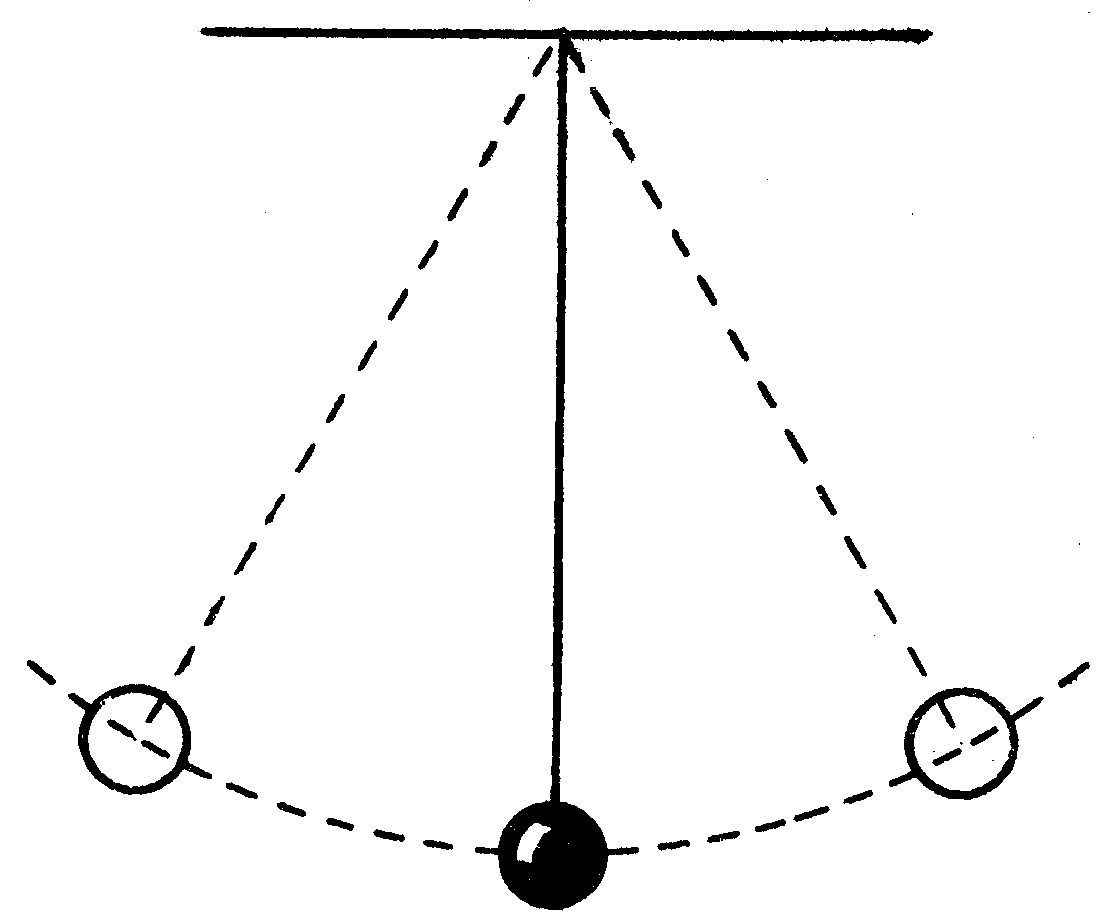
\includegraphics[scale=0.3]{mayat.png}
	\caption {Модель маятника}
	\label{fig:pend}
\end{figure}

%%%%%%%%%%%%%%%%%%%%%%%%%%%%%%%%%%%%%%%%%%%%%%%%%%%%%%%%%%%%%%%%%%%%%%%%%%%%%%%%
\section{Управление по прогнозируемой модели (MPC)}\label{1sec:mpc}
%%%%%%%%%%%%%%%%%%%%%%%%%%%%%%%%%%%%%%%%%%%%%%%%%%%%%%%%%%%%%%%%%%%%%%%%%%%%%%%%


Управление по прогнозирующей модели, в англоязычной литературе носящее название Model Predictive Control (MPC), является одним из современных методов теории управления \cite{mpcIn, mpcIn2}. Подход управления с прогнозирующими моделями начал развиваться в начале 60-х годов XX века для управления процессами и оборудованием в нефтехимическом и энергетическом производстве, для которых применение традиционных методов синтеза было крайне затруднено в связи с исключительной сложностью их математических моделей. В последнее время область применения MPC значительно расширилась, охватывая технологические отрасли и экономику при управлении производством, при решении задач управления запасами и портфелем ценных бумаг. 

Основным достоинством MPC-подхода, определяющим его успешное использование в практике построения и эксплуатации систем управления, служит относительная простота базовой схемы формирования обратной связи, сочетающаяся с высокими адаптивными свойствами. Последнее обстоятельство позволяет управлять многомерными и многосвязными объектами со сложной структурой, оптимизировать процессы в режиме реального времени в рамках ограничений на управляющие и управляемые переменные, учитывать неопределенности в задании объектов и возмущений. Кроме того, возможен учет запаздываний, поскольку зачастую решение об управлении принимается в момент времени t – h, а реализация этого решения происходит в момент времени t. Классической областью применения MPC до недавнего времени были задачи стабилизации и слежения в технических приложениях. Теоретические основы метода для задач стабилизации получили строгое обоснование в работах \cite{mpcIn, mpcIn2}.

MPC основывается на последовательном, в каждый момент времени, решении прогнозирующих задач оптимального управления (predictive optimal control problems) с конечным горизонтом управления, сформулированных для математической модели управляемого объекта, начальное условие которой совпадает с измеренным состоянием объекта. Значение оптимального программного управления прогнозирующей задачи на левом конце промежутка управления используется для управления объектом в текущий момент времени и до тех пор, пока не будет получено и обработано следующее измерение состояния.

Управление, которое подается на объект в описанном процессе, представляет собой \textit{обратную связь} (оно зависит от измеряемых состояний), свойства которой зависят от конкретного вида прогнозирующей задачи оптимального управления и целей управления объектом (например, стабилизация, регулирование, слежение и др.).

Методы МРС предполагают построение стабилизирующей обратной связи на основе повторяющегося в каждый текущий момент времени решения задач оптимального управления (ОУ)\cite{mpc}. Для того, чтобы учесть практическую невозможность мгновенного вычисления решения задач ОУ, предполагается, что состояния среды обрабатываются (измеряются) в дискретные моменты времени $\tau \in \{0, h, 2h, \dots\}$, где $h > 0$ – период квантования,
превосходящий время решения задач ОУ. Соответственно, будет строиться дискретная обратная связь, что позволяет определить решение замкнутой системы при заданном начальном состоянии как последовательное решение уравнения
(\ref{eq:diff}), $x(\tau) = x(\tau - 0) $ на интервалах $t \in [\tau, \tau + h[$.

Общая идея МРС состоит в решении в каждый момент $\tau$ так называемой прогнозирующей задачи ОУ с конечным горизонтом $T = Nh$ ( $N$ – натуральное число), в которой начальное условие для прогнозирующей модели совпадает с измеренным состоянием $x(\tau)$ объекта управления. В качестве прогнозирующей модели выбирается математическая модель объекта управления, которая может отличаться: это может быть линеаризация,
или детерминированная модель, в которой не учитываются возмущения, немоделируемая динамика, другие неопределенности. 

Базовый алгоритм МРС состоит в следующем: для каждого $t$ выполнить
\begin{enumerate}
	\item измерить текущее состояние $x(t)$ объекта управления;
	\item решить задачу, получить оптимальное программное управление $u$
	\item подать в среду управляющее воздействие.
\end{enumerate}

Построенная в результате применения данного алгоритма функция 
$u_{MPC} (t),$  $ t \ge 0$ , является реализацией дискретной обратной связи вида $u = u^0(\tau)$ , вдоль траектории измерений, реализовавшейся в конкретном процессе управления.  Она обеспечивает асимптотическую устойчивость решения замкнутой системы при ряде дополнительных условий. В частности, известно, что при недостаточно больших горизонтах управления $T$ система может оказаться неустойчивой, поэтому авторами \cite{mpcIn2} получены нижние оценки параметра $T$, гарантирующие асимптотическую устойчивость. Нужно отметить,
что при таком подходе горизонт управления может оказаться достаточно большим, что отрицательно скажется на трудоемкости решения задачи.

 Исторически первый подход состоит в том, чтобы дополнить задачу  терминальным ограничением. Недостатками данного подхода являются: 1) при коротких горизонтах планирования прогнозирующая задача ОУ может не иметь решения, 2) двухточечные задачи ОУ являются самыми сложными с вычислительной точки зрения. Устраняют перечисленные недостатки подходы \cite{mpcIn2}, в которых задача дополняется
терминальным ограничением , выбирается критерий качества типа Больца (\ref{eq:bolt}). Асимптотическая устойчивость замкнутой системы в подходах \cite{mpcIn2} гарантируется в том случае, если существует некоторое множество $S$, на котором найдется такая локальная обратная связь $U$, что: 1) множество $S$ является положительно инвариантным для системы $\ddot{x} =  f (x, k (x)), x \in S$ ; 2) при всех $x \in S$ имеет место включение $k(x) \in U$ .

В рамках поставленной задачи (\ref{eq:main}) необходимо найти последовательность управлений $u = \{u_0, \dots , u_{N-1} \}, u_i \in [-2, 2]$, в результате чего будет достигнуто максимальное значение критерия качества. То есть если задано начальное состояние $\overline{x_0}\in \mathbb{R^n}$, то с помощью управления по прогнозирующей модели в каждый момент времени $k=\overline{1, N}$ находится последовательность управляющих воздействий  с горизонтом планирования $T$: $\{u'_0, \dots , u'_{T-1}\}, u'_i \in [-2, 2]$, в систему подается управление $u_k = u'_0$, возвращается ее будущее состояние и заново перестраивается последовательность управлений с  горизонтом планирования $T$. Таким образом находится траектория решения задачи:

$$x(\overline{x_0}, u) ,$$
соответствующая начальному состоянию $x_0$ и последовательности управлений $u$.

%%%%%%%%%%%%%%%%%%%%%%%%%%%%%%%%%%%%%%%%%%%%%%%%%%%%%%%%%%%%%%%%%%%%%%%%%%%%%%%%
\section{Выводы}\label{1sec:conc}
%%%%%%%%%%%%%%%%%%%%%%%%%%%%%%%%%%%%%%%%%%%%%%%%%%%%%%%%%%%%%%%%%%%%%%%%%%%%%%%%

В рамках данной главы была представлена общая характеристика и рассмотрена классификация задач оптимального управления. На основе чего была выбрана и поставлена задача, решаемая в рамках данной работы. Также были рассмотрены основные принципы и классификация методов машинного обучения. В результате из всех разновидностей выбран метод обучения с подкреплением для решения поставленной задачи. Также дан обзор управления по прогнозируемой модели. Более подробно он рассматривается в следующей главе.
